\documentclass[11pt]{article}

%stuff for math
\usepackage{amssymb}
\usepackage{amsthm}
\usepackage{amsmath}
\usepackage{mathtools}

%stuff for graphics
\usepackage{caption}
\usepackage{subcaption}
\usepackage{graphicx}

%enumeration add-on
\usepackage{enumerate}

%margin stuff
\usepackage[top=0.75in, bottom=0.75in, left=1.75in, right=1.75in]{geometry}

\begin{document}

\author{David Goulette}
\title{Introduction to learning \LaTeX}
\maketitle
\section{Introduction}
Hello \LaTeX\ learners!  I just want to say right from the outset that I am not an expert in \LaTeX.  I am just a fairly experienced user.  So my goal is not to teach the really advanced stuff to you (some advanced things I know how to do because I needed it for my work, but there are tons of advanced things that I have no idea how to do).  I just want you to know how to do the basics and also learn how to teach yourself the more advanced things if and when you need them.  So I will help get you past the initial learning curve and I will also give you the resources to learn more on your own.  Once you understand the basics, you will be able to learn more advanced things fairly easily.

Now, you might be wondering what \LaTeX\ is and why it is useful. Well, one great thing about \LaTeX\ is that it is open source, which means that it is free\footnote{I mean free as in ``free speech'' and also free as in ``free beer.''  So \LaTeX\ doesn't cost anything \emph{and} you can modify it however you like \emph{and} you can pass the modifications on to whomever you want.}.  But more importantly, it is the standard software used to create professional quality technical documents.   It is used by mathematicians, statisticians, scientists, engineers, physicists, etc. The great thing about \LaTeX\ is that it gives you the ability to easily add mathematics and symbols to your document. But \LaTeX\ also looks much better than Microsoft Word or other similar word processors. Also, entering math and getting it to look really professional is \emph{much} faster in \LaTeX\ than any other document preparing software.  For example, if I want to include the binomial theorem in my paper, then it is very easy once you get comfortable with the commands needed to do it. Here is the binomial theorem:
\[
(x+y)^n=\sum_{i=0}^{n} \binom{n}{i} x^{n-i}y^i.
\]
And it took me less than a minute to type the commands needed to get that equation. If you try to do that in Microsoft Word it will take you a while to get it and it won't look as good.

Unfortunately many people don't learn how to use \LaTeX\ because it can be a little challenging at first.  But it is my goal to help you get past the initial challenges. And once you learn the basics, it is really easy to make basic documents. Once you are comfortable with the basics, then the sky is the limit.  You can use it to do homework, write essays, articles, letters, a PhD. thesis, or even write your own book\footnote{But unfortunately \LaTeX\ won't help you find a publisher... that is up to you.  By-the-way, footnotes like this one are extremely easy to make}.

\section{Resources}
The three main websites that you need to know about are the following (I will explain what you will find at each of these below):
\begin{enumerate}
\item \verb|www.ctan.org|
\item \verb|www.sjsu.edu/people/david.goulette/courses/latex/|
\item \verb|http://en.wikibooks.org/wiki/LaTeX|
\end{enumerate}
\subsection{Where to get \LaTeX}
So the first thing you need to do to be able to learn \LaTeX\ is to get it installed on your computer so you can start playing with it. The place to go is the first link listed above.  CTAN stands for Comprehensive TeX Archive Network.  CTAN is essentially the online repository for all of the packages that can be added to the basic \LaTeX\ installation\footnote{Although the basic installation of \LaTeX\ is very powerful, there are some things it can't do easily.  But people have developed literally \emph{thousands} of free add-on packages that will allow you to do tons of really cool stuff.  I will teach you how to use some useful packages.}.  They also have documentation on how to use those add-on packages  But they also have links to current distributions of \LaTeX\ for you to install.  The version you need to install depends on which operating system you have on your computer.  The three main \LaTeX\ distributions that I recommend are called \TeX\,Live (for Linux), Mac\TeX\, (for Mac), and Pro\TeX t (for Windows). (Just so you know, if you have a Windows operating system, when you install Pro\TeX t you are \emph{actually} installing something called Mik\TeX. Pro\TeX t is just an easy-to-install version of Mik\TeX\, that comes bundled with some very useful extra tools.  So when you install Pro\TeX\, it will be called Mik\TeX\, in your list of programs.)  When you go to CTAN's website, look on the right hand side of the page for what you see in this picture:\\
\begin{center}
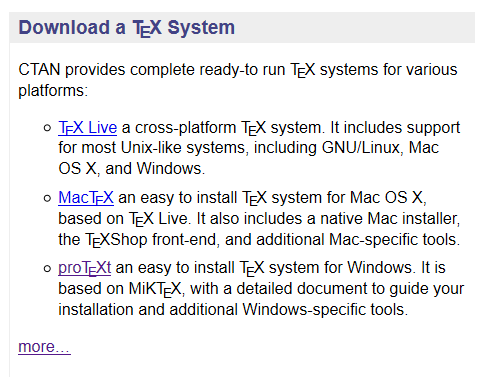
\includegraphics[width=.6\columnwidth]{Capture}
\end{center}
Just click on the appropriate version for your operating system and follow the instructions.  You will have to download an installer which might be a fairly large file (the Windows version is 1.6 gigs so it will take a while to download).  During the installation process there will likely be two questions that will come up in a pop-up window that could be a bit confusing to you. The first will be to choose your ``preferred paper.''  Now, the default choice will probably be A4.  You might not have heard of it before, but A4 is the name for a size of paper that is $210\times 297$ millimeters in size.  A4 is a standard paper size in many European countries.  But you will want to change that option to ``Letter'' which is the 8.5 by 10 inch standard in the U.S. The other option you will need to choose is whether or not your \LaTeX\ distribution will ``install missing packages on the fly'' (or it will say something similar to that).  Choose either ``Yes'' or ``Ask me first.''  You want to be able to add free add-on packages easily and this will make it so that they are installed for you without you doing any of the dirty work.  Now, to be honest, I have never installed the Mac or Linux versions so I am not sure if it will ask these questions just as I have stated it here, but I am assuming it will \emph{probably} ask you these questions or something similar.  Contact me if you have issues and I will try my best to help.

\subsection{Other resources}
The second link that I listed above is on my faculty website. This is the where I am planning to post links to various \LaTeX\ resources like videos, templates and examples. You will find this document there as well. I will post links to free online resources that will substitute for a textbook.  In fact, you can learn anything you want to know about \LaTeX\ for free online (that is how I learned everything I know about \LaTeX). But for now I want you to download ``The Non So Short Introduction to \LaTeXe'' by Tobias Oetiker. It can be found at 
\begin{center}
\verb|http://tobi.oetiker.ch/lshort/lshort-letter.pdf|
\end{center}
He has written a fantastic introduction to \LaTeX\ that is very easy to read.  I will likely be assigning some reading from his introduction later.  If you are really excited to get started reading this and learning \LaTeX\ on your own then, by all means, start reading it now!

The third link listed above is an ever growing wikibook that can be very useful.  But it can be a little overwhelming because they often have very detailed information.  But once you have some of the basics down, this wikibook is a great place to learn various skills.  

The last resource for learning \LaTeX\ that I will mention is google.  If you just search for whatever you are trying to figure out, you will likely find something that is helpful. Often somebody has posted something on \verb|tex.stackexchange.com| or other similar sites that have open discussion regarding \LaTeX\ issues.
\end{document}
